\section{Błażej Brudnowski}
\subsection{Wyrażenie matematyczne}

\begin{align}
{e^{(i * \pi)} + 1 = 0}
\pagenumbering{gobble}
\end{align}


\begin{itemize}
\subsection{Itemy}
\item[1]{Punkt pierwszy}
\item[2]{Punkt drugi}
\end{itemize}


\begin{itemize}
\subsection{Itemy}
\item[]{Punkt pierwszy}
\item[]{Punkt drugi}
\end{itemize}


\begin{center}
\subsection{Text}
this text is cool


this text is cooler

\textbf{the coolest}

\underline{decent of the coolest}


\begin{table}
\subsection{Tabela}
\begin{tabular}{|l|l|l|l|l|}
1 & 1 & 1 & 1 & 1 \\
1 & 1 & 1 & 1 & 1 \\
1 & 1 & 1 & 1 & 1 \\
1 & 1 & 1 & 1 & 1 
\end{tabular}
\caption{tabela}
\end{table}


\begin{figure}
    \subsection{Obraz}
    \centering
    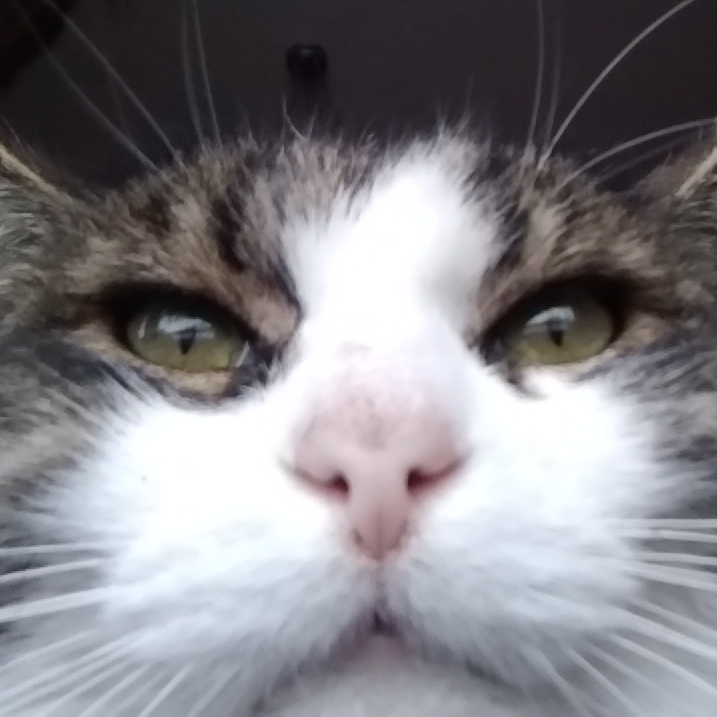
\includegraphics[width=0.5\linewidth]{pictures/kat.png}
    \caption{Kat}
    \label{The cat}
\end{figure}


\end{center}